\documentclass[12pt,a4paper]{ufpr}

\usepackage[brazil]{babel}
\usepackage[utf8]{inputenc}
\usepackage{amssymb,amsmath}
\usepackage{epsfig}
\usepackage{multirow}
\usepackage{amssymb}
\usepackage{graphicx}
\usepackage{setspace}
\usepackage{ps-macros}
\usepackage[linktocpage=true]{hyperref}
\usepackage{makeidx}
% \usepackage{caption2}
\usepackage{caption}
\usepackage{subcaption}

\usepackage{algorithm}
\usepackage{algpseudocode}

\floatname{algorithm}{Algoritmo}
\renewcommand\algorithmicend{\textbf{fim}}
\renewcommand\algorithmicdo{\textbf{faça}}
\renewcommand\algorithmicwhile{\textbf{enquanto}}
\renewcommand\algorithmicfor{\textbf{para}}
\renewcommand\algorithmicforall{\textbf{para todo}}
\renewcommand\algorithmicif{\textbf{se}}
\renewcommand\algorithmicthen{\textbf{então}}
\renewcommand\algorithmicelse{\textbf{senão}}
\renewcommand\algorithmicreturn{\textbf{retorne}}
\algnewcommand\algorithmicforeach{\textbf{para cada}}
\algdef{S}[FOR]{ForEach}[1]{\algorithmicforeach\ #1\ \algorithmicdo}%

\setcounter{secnumdepth}{3}    % n - numero de niveis de subsubsection numeradas
\setcounter{tocdepth}{3}       % coloca ate o nivel n no sumario

\title{A ser definido}
\author{Eduardo Luís Buratti}
\advisortitle{Orientador}
\advisorname{Prof. Dr. Eduardo Jaques Spinosa}
\advisorplace{Departamento de Informática, UFPR} % departamento, instituicao
\city{Curitiba}
\year{2013}

% \banca        % nao insira o nome do orientador, ja eh feito automaticamente
% {Prof. Dr. Luciano Fontoura}{Instituto de Física, USP}
% {Prof. Dr. Hélio Pedrini}{Departamento de Informática, UFPR}
% {Prof. Dr. Alexandre I. Direne}{Departamento de Informática, UFPR} % se nao houver deixe em branco {}{}
% {}{}    % se houver um quarto membro na banca, inserir nome e instituicao
% \defesa{04 de outubro de 2000} % dia em que foi realizada a defesa da dissertacao

\makeindex

\begin{document}

\pdfstringdefDisableCommands{%
    \let\MakeUppercase\relax
}

\makecapamonografia
\makerostomonografia
% \maketermo

%\singlespacing
%\onehalfspacing
\doublespacing

\pagestyle{headings}
\pagenumbering{roman}

% \chapter*{Agradecimentos}
% Agradeço primeiramente a meus pais pelo apoio e suporte que me permitiram chegar até aqui.\\

\noindent
Aos meus dois irmãos e irmã pelo exemplo e inspiração que formaram meu caráter.\\

\noindent
Ao meu professor orientador por dedicar parte de seu tempo para me guiar e motivar a cada passo deste trabalho.\\

\noindent
Aos meus amigos e colegas de trabalho pela compreensão e apoio nos momentos mais necessários.\\

\noindent
E a todos que contribuíram de forma direta ou indireta para a minha jornada, espero poder retribuir de alguma forma no futuro.

\chapter*{Resumo}
\addcontentsline{toc}{chapter}{RESUMO}
Texto do resumo....

\newpage

\chapter*{Abstract}
\addcontentsline{toc}{chapter}{ABSTRACT}
Among several living beings observed in nature, those with self-organization capabilities stand out. In a collective way, these living beings can overcome their own physical and cognitive limitations in order to solve more complex and difficult tasks. Swarm robotics is an area of robotics concentrated into the apllication of similar concepts to solve problems in the robotics area. This work aims to evaluate several strategies and algorithms (utilizing evolutionary robotics) for synthesis of an autonomous robot controller whose purpose is to reproduce the path-formation collective behavior.\\

\noindent
Keywords: Swarm Robotics, Evolutionary Robotics, Path Formation.
\newpage

\listoffigures
\addcontentsline{toc}{chapter}{LISTA DE FIGURAS}
\newpage

\listoftables
\addcontentsline{toc}{chapter}{LISTA DE TABELAS}
\newpage

\tableofcontents
\addcontentsline{toc}{chapter}{SUMÁRIO}
\newpage

\pagenumbering{arabic}

\chapter{Introdu\c{c}\~ao}
\label{Introducao}

Teste para a introdu��o da disserta��o, refer�ncia\cite{tese1,artigo1}

\section{Novo}

Teste para a introdu��o da disserta��o, refer�ncia\cite{tese1,artigo1}



% *****************
% O [41] determina o percentual de reducao em relacao ao tamanho original.
% *****************
% \begin{figure}
% \centerfig{feature_space_2D.ps}[41]
% \caption{Legenda geral da figura.}
% \label{figura_xpto}
% \end{figure}
% *****************



Teste para a introdu��o da disserta��o, refer�ncia\cite{tese1,artigo1}
Teste para a introdu��o da disserta��o, refer�ncia\cite{tese1,artigo1}
Teste para a introdu��o da disserta��o, refer�ncia\cite{tese1,artigo1}
Teste para a introdu��o da disserta��o, refer�ncia\cite{tese1,artigo1}
Teste para a introdu��o da disserta��o, refer�ncia\cite{tese1,artigo1}
Teste para a introdu��o da disserta��o, refer�ncia\cite{tese1,artigo1}




% *****************
% O .50 da minipage e' para dividir a largura da pagina em 2 figuras por
% linhas, se for colocar 3 subfiguras por linha .33 e assi vai...
% a largura da imagem e' 3cm.(width=3cm).
%
% O (!ht) e' para forcar o latex a colocar a figura na posicao, ou
% paragrafo onde foi inserido no texto o \begin{figure}, "se possivel"
% e' claro...
% *****************
% \begin{figure}[!ht]
% \renewcommand{\captionfont}{\it}
% \renewcommand{\captionlabelfont}{\bf}
% \begin{minipage}[b]{.50\textwidth}
% \centering
%   \subfigure[Imagem 1]{
%     \label{fig:teste:a}
%     \includegraphics[width=3cm]{feature_space_2D.ps}}
% \end{minipage}%
% \begin{minipage}[b]{.50\textwidth}
% \centering
%   \subfigure[Imagem 2]{
%     \label{fig:teste:b}
%     \includegraphics[width=3cm]{feature_space_2D.ps}}
% \end{minipage}
% \caption{
%   Legenda geral da figura contendo 2 sub-figuras colocadas lado a lado.}
% \label{fig:teste}
% \end{figure}
% *****************


Teste para a introdu��o da disserta��o, refer�ncia\cite{tese1,artigo1}
Teste para a introdu��o da disserta��o, refer�ncia\cite{tese1,artigo1}
Teste para a introdu��o da disserta��o, refer�ncia\cite{tese1,artigo1}
Teste para a introdu��o da disserta��o, refer�ncia\cite{tese1,artigo1}
Teste para a introdu��o da disserta��o, refer�ncia\cite{tese1,artigo1}
Teste para a introdu��o da disserta��o, refer�ncia\cite{tese1,artigo1}


% *****************
% \begin{figure}
% \psfig{file=feature_space_2D.ps,height=2in,width=3.5in}
% \caption{Legenda geral da figura usando psfig COM reducao.}
% \end{figure}
% *****************

Teste para a introdu��o da disserta��o, refer�ncia\cite{tese1,artigo1}
Teste para a introdu��o da disserta��o, refer�ncia\cite{tese1,artigo1}
Teste para a introdu��o da disserta��o, refer�ncia\cite{tese1,artigo1}
Teste para a introdu��o da disserta��o, refer�ncia\cite{tese1,artigo1}
Teste para a introdu��o da disserta��o, refer�ncia\cite{tese1,artigo1}
Teste para a introdu��o da disserta��o, refer�ncia\cite{tese1,artigo1}


% *****************
% \begin{figure}
% \psfig{file=feature_space_2D.ps}
% \caption{Legenda geral da figura usando psfig SEM reducao.}
% \end{figure}
% *****************

\chapter{Robótica evolutiva}
\label{evolutiva}

\section{Introdução}

introdução

\section{Redes Neurais Artificiais (RNA)}

Redes neurais artificias são sistemas computacionais inspirados em sistemas
nervosos animais capazes de aprendizado. Matematicamente, RNAs são aproximadores
universais \cite{hornik89universal}. Um RNA é composto por uma rede de unidades
de processamento simples (neurônios). Cada neurônio possui um sinal de saída e
pode receber um ou mais sinais de entrada.

\subsection{Multi-Layer Perceptron (MLP)}

Uma rede neural MLP é composta por uma série de neurônios organizados em camadas, onde cada neurônio recebe, como entrada, a saída dos neurônios da camada anterior. Uma rede com uma camada intermediária é capaz de aproximar qualquer função contínua. Com duas camadas intermediárias, qualquer função pode ser aproximada \cite{cybenko89mlp}.

\begin{figure}[h]
    \centering
    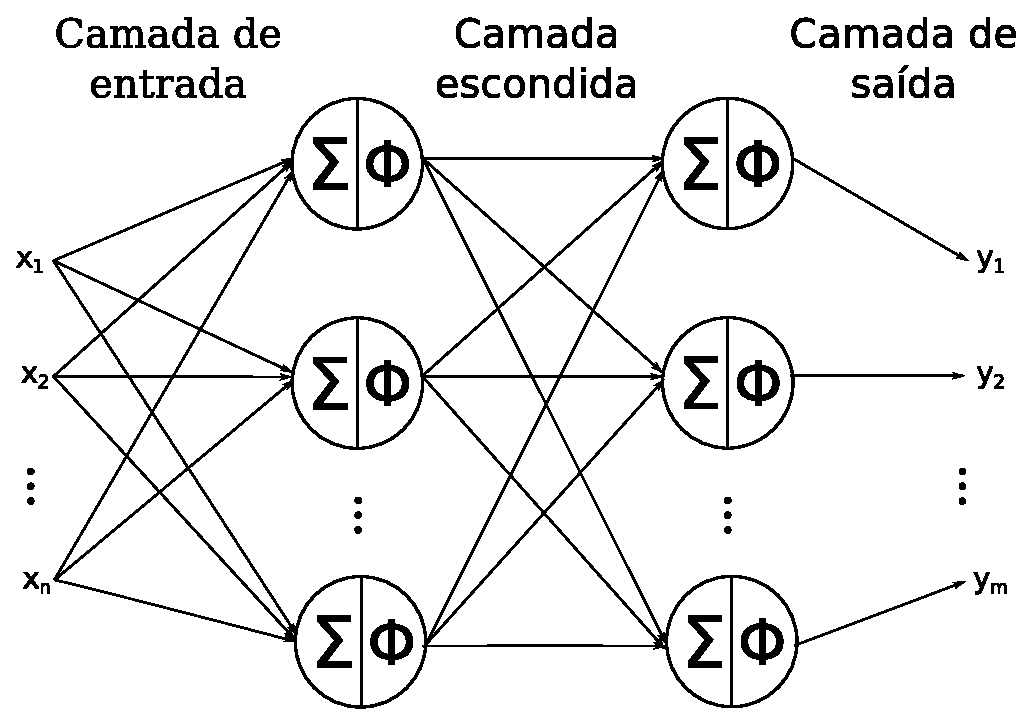
\includegraphics[width=0.4\textwidth]{figures/mlp}
    \caption{Multi-layer Perceptron}
    \label{fig:mlp}
\end{figure}

A saída (y) de um neurônio é determinada pela aplicação de uma função de ativação \(\theta\) sobre a combinação linear ponderada de todas as suas \(n\) entradas \((x_1, x_2, \dots , x_n)\).

Matematicamente,

\[ y = \theta ( \sum_{i=1}^{n} w_i x_i ) \]

onde \(w_i\) é um peso associado a entrada \(i\).

Diversas funções pode assumir o papel de função de ativação, sendo as mais comuns:
a função degrau (\ref{eq:degrau}) e a função sigmóide (\ref{eq:sigmoid}).

\begin{equation} \label{eq:degrau}
    \theta(x) = \left\{
    \begin{array}{l l}
        0 & \quad \text{se } x < 0\\
        1 & \quad \text{caso contrário}
    \end{array} \right.
\end{equation}

\begin{equation} \label{eq:sigmoid}
    \theta(x) = \frac{1}{1 + e^{-x}}
\end{equation}

É comum encontrar, em cada uma das camadas, um neurônio adicional cuja entrada é sempre \(1\). Este neurônio especial tem o nome de \textit{bias} e a finalidade de deslocar a função de ativação para direita ou esquerda.

O ajuste dos pesos \((w_1, w_2, \dots , w_n)\) é chamado treinamento e existe em duas formas:

\begin{description}
    \item[Supervisionado]: É fornecido ao algoritmo de treinamento um conjunto de entradas/saídas. O algoritmo iterativamente ajusta os pesos da rede a fim de que, dadas entradas do conjunto de treinamento, as saídas da rede aproximem-se das saídas.
    \item[Não supervisionado]: Não demanda conjunto de treinamento, os pesos
são ajustados considerando a aptidão da rede à solução do problema.
\end{description}

\subsection{Time-Delay Neural Network (TDNN)}

Estendendo os conceitos das redes MLP, uma TDNN permite à cada neurônio armazenar um
histórico dos sinais de entrada. Isto permite que a rede ganhe sensibilidade à padrões temporais, ou seja, a rede pode adaptar-se não só à padrões como também à sequência de padrões \cite{kaiser94tdnn}.

Este modelo de rede neural é de especial importância na área de robótica. As ações determinadas pelo controlador de um robô devem levar em conta o histórico sensorial e não apenas o estado sensorial atual.

\section{Controle de robôs móveis por RNA}

% ann as robot controller

% [zhang 2000]
% Although many types of neural networks can be used
% for classification purposes [105], our focus nonetheless is on
% the feedforward multilayer networks or multilayer perceptrons
% (MLPs) which are the most widely studied and used neural net-
% work classifiers.

\section{Algoritmos de otimização para treinamento de RNA}
\label{optimization-algorithms}

ga, pso, dpso, bpso, pga
\chapter{Robótica de enxame}
\label{swarm}

\section{Introdução}

\section{Inteligência coletiva}

Observando os seres vivos presentes na natureza, podemos facilmente extrair algumas qualidades que estes apresentam: flexibilidade, robustez, descentralização, auto-organização. Em grande parte, o motivo por trás dessas qualidades é a coletividade. Por exemplo, em colônias de insetos sociais, diversos indivíduos se auto-organizam para realizar tarefas cuja  escala e complexidade superam, e muito, os limites físicos e cognitivos de cada indivíduo. Podemos visualizar uma colônia como um único super-organismo [Trianni 2011] e podemos interpretar inteligência como uma característica que emerge das interações entre componentes simples e interdependentes de um sistema.

Sob esse ponto de vista, uma série de algoritmos computacionais têm sido propostos em
uma área de pesquisa denominada inteligência coletiva (\textit{swarm intelligence}) [Bonabeau 1999]
[Kennedy 2001]. De forma análoga, robótica de enxame (\textit{swarm robotics}) também utiliza dos mesmos conceitos para resolução de diversos problemas da área de robótica.

Diversos algoritmos bioinspirados de inteligência coletiva vem sendo propostos [Bonabeau 1999] [Kennedy 2001] e avaliados no contexto da robótica de enxame [Navarro 2013]. Com eles é possível produzir vários comportamentos coletivos. Alguns relativamente simples e outros bastante mais complexos, que em geral dependem da execução coordenada de alguns dos comportamentos coletivos simples.

O comportamento de agregação, por exemplo, consiste simplesmente na reunião dos
robôs do enxame e é utilizado por outros comportamentos complexos, como o movimento
coletivo, a auto-montagem e a formação de padrões, nos quais em determinados momentos o
enxame se reúne.

No comportamento de dispersão, o enxame se distribui de modo a ocupar a maior área
possível do espaço sem perder comunicação. É útil em tarefas que envolvam a exploração
coletiva de um território desconhecido.

A formação de padrões é um comportamento em que os robôs devem movimentar-se de
maneira coordenada para distribuírem-se no espaço segundo um determinado modelo de
posicionamento.

Já no comportamento de movimento coletivo o enxame deve mover-se em conjunto e de
maneira coesa [Sperati 2008]. Há, nesse caso, uma clara inspiração na natureza, por exemplo na
maneira como se movimentam pássaros em um bando ou peixes em um cardume. Pelo menos
dois tipos de movimento coletivo podem ser identificados: formation, em que o posicionamento e a
orientação dos robôs mantêm-se fixa, e flocking, em que isso não acontece.

O comportamento de busca por alimento (foraging) observado na natureza pode inspirar
uma gama mais ampla de problemas em que os robôs devem encontrar as coordenadas de um
ponto do ambiente com características definidas.

A formação de caminho é uma variação de movimento coletivo que também se enquadra em busca por alimento. Visa o trajeto do enxame pelo menor caminho entre dois pontos, assim como, na natureza, as formigas utlizam de feromônios para encontrar e navegar pelo menor caminho entre o formigueiro e alguma fonte de alimento.

Alocação de tarefas é um comportamento genérico que se aplica a diversos problemas em
que o enxame precisa, de maneira coletiva e descentralizada, definir a tarefa que cabe a cada
robô. Trata-se de um problema relativamente complexo em que diversos estudos vêm sendo
realizados.

O transporte coletivo de objetos é outro comportamento facilmente observável na natureza,
por exemplo em colônias de formigas. Envolve alto grau de coordenação e depende de vários
dos comportamentos básicos mais simples [Gross 2006].

Um comportamento com importante aplicação na exploração de ambientes desconhecidos
é o do mapeamento coletivo, em que o comportamento de dispersão é associado à troca de
informações entre robôs com o objetivo de produzir uma representação mais ampla do ambiente.

Outro comportamento relativamente complexo é a auto-montagem [Christensen 2007], que
consiste na agregação e interconexão de robôs formando padrões que podem ser posteriormente
utilizados para a solução coletiva de problemas.

\section{Formação de caminho}

Da observação do comportamento de diversas espécies de formigas, nota-se o uso de químicos (feromônios) para estabelecer uma forma de comunicação que permite: o recrutamento em massa de indivíduos e a formação dinâmica de um caminho para transporte do alimento para dentro da colônia.

No contexto de robótica de enxame, Fujisawa et al. \cite{fujisawa2008pheromone} recria com sucesso esse comportamento em um grupo de robôs. No entanto, a síntese, armazenamento, fator de evaporação e detecção confiável dos quimícos não é nada simples e dificulta o uso prático de tal método.
Por outro lado, diversas abordagens ao problema procuram alternativas aos feromônios, por exemplo: projeção luminosa [], \textit{RFID} [], trilhas virtuais [] etc.

Neste trabalho focaremos no seguinte problema: recriar o comportamento de formação de caminho de forma eficiente (menor caminho) entre duas áreas alvo por um enxame de robôs. A posição das áreas alvo são, inicialmente, desconhecidas pelos agentes. O robô é capaz de mover-se livremente dentro de um espaço retangular limitado por paredes. Outros robôs e as paredes são sensíveis à sensores presentes em cada robô. Os agentes também são capazes de identificar e emitir luzes para estabelecer alguma forma de comunicação. Contudo, explorando o alcance limitado dos sensores, as áreas alvo são posicionadas a fim de impedir que ambas áreas sejam percebidas, ao mesmo tempo, por um mesmo agente.
\chapter{Contorno do problema e o ambiente de simulação}
\label{cha:problem-limits}

\section{Introdução}

Como Sperati et al. [\cite{sperati2011path}], abordamos o problema de formação de caminho utilizando robótica evolutiva. Cada robô é controlado por uma \textit{Time-Delay Neural Network} (Seção \ref{sec:tdnn}) e seus parâmetros (total de 113 pesos) são ajustados por algoritmos evolutivos (Seção \ref{sec:evolutionary-computation}).

A Seção \ref{sec:robots} descreve o robô utilizado para os estudos. A Seção \ref{sec:environment} descreve o ambiente a que esses robôs são submetidos. A Seção \ref{sec:fitness} define a função de \fitness que avalia a qualidade de uma solução para a instância do problema em questão. Por fim, a Seção \ref{sec:simulation} apresenta o ambiente de simulação desenvolvido e a motivação para tal feito.

\section{Os robôs}
\label{sec:robots}

O robô utilizado como referência é o \textit{e-puck} \cite{mondada2009epuck}, um pequeno robô cilíndrico com 7 centímetros de diâmetro. Dois motores independentes controlam duas rodas provendo tração diferencial e velocidade de até 8.2 cm/s. Oito sensores de luz infravermelha ao redor do robô permitem a detecção de obstáculos próximos (até aproximadamente 2.5 cm). Mais um sensor de luz infravermelha é colocado em baixo do robô para detecção da cor do chão (usado para diferenciar as áreas alvo do resto do ambiente). Além disso, o robô possuí uma câmera com alcance de 35 cm e campo de visão de $144\,^{\circ}$. Dois LEDs\footnote{\textit{Light-Emitting Diode} -- Diodo emissor de luz} de cores diferentes na dianteira e traseira do robô, podendo ser acessos ou apagados, são detectáveis pela câmera de outros robôs permitindo uma forma de comunicação.

Para representar a informação captada pela câmera a codificamos em quatro valores binários: presença ou não de pontos azuis ou vermelhos (correspondendo aos LEDs dianteiros e traseiros, respectivamente) na região direita ou esquerda do campo de visão.

A estrutura da rede neural pode ser vista na Figura \ref{fig:robot-ann}. O conjunto de entradas da rede é composto por todos os sensores do robô devidamente normalizados (total de 13 entradas) e o conjunto de saídas controla os dois motores e os dois LEDs (total de 4 saídas). Vale observar que a configuração da rede (estrutura e pesos) é homogênea à todos os robôs do enxame, ou seja, cada robô possuí sua própria rede neural funcionando de forma independente porém a configuração da rede é igual para todos os robôs de um enxame durante um experimento.

\begin{figure}[H]
    \centering
    \includegraphics[width=0.8\textwidth]{figures/robot-ann}
    \caption{Rede neural controladora do robô}
    \label{fig:robot-ann}
\end{figure}

Matematicamente, a ativação $O_{j}$ do neurônio de saída $j$ no momento $t$ é computado pelas seguintes equações:

$$
O_{j}(t) = \sigma (\sum_{i} w_{ij}^{OI} I_{i}(t) + \sum_{i} w_{ij}^{OH} H_{i}(t) + \beta_{j}^{O})
$$
$$
H_{j}(t) = \tau_{j} \sigma (\sum_{i} w_{ij}^{HI} I_{i}(t) + \beta_{j}^{H}) + (1 - \tau_{j}) H_{j} (t - 1)
$$

onde $I_{i}$ é o valor da entrada $i$ (sensor normalizado). $\beta_{j}^{H}$ e $\beta_{j}^{O}$  representam o \textit{bias} relativo ao neurônio $j$ da camada intermediária e de saída, respectivamente. Finalmente, $w_{ij}^{OI}$, $w_{ij}^{OH}$ e $w_{ij}^{HI}$ são os pesos relativos a entrada $i$ e saída $j$ das sinapses que ligam, respectivamente, os neurônios: de entrada para saída, de entrada para intermediários e intermediários para saída.

O parâmetro denominado \textit{time constraint} ($\tau_{j}$) determina a fração de ativação do neurônios da camada escondida no momento anterior $H_{j} (t - 1)$ que é mantida no momento atual $H_{j} (t)$. Isso classifica a rede como uma \textit{Time-Delay Neural Network} visto que o histórico de ativação das entradas têm alguma influência na saída.

\section{O ambiente}
\label{sec:environment}

Os robôs são colocados em um espaço quadrado (250 cm de lado) delimitado por paredes. Dentro desse espaço, duas circunferências (16 cm de raio), denotadas por uma coloração escura (em contraste ao restante do espaço que apresenta coloração mais clara), representam as áreas alvo. O sensor de luz infravermelha localizado em baixo do robô é sensível à diferença de coloração, podendo assim perceber se está sobre uma área alvo ou não. Adicionalmente, no centro das áreas alvo, dois LEDs vermelhos sempre acessos são visíveis, indistinguivelmente, como os LEDs na traseira dos robôs.

\section{A função de \fitness}
\label{sec:fitness}

Seguindo o mesmo conceito apresentado por Sperati et al. \cite{sperati2011path}, a \fitness $F$ de uma solução $S$ é computada a partir de um teste com os robôs no ambiente físico por um determinado intervalo de tempo $T$. Dividimos esse intervalo em duas partes $T_{a}$ e $T_{b}$. Durante a primeira parte, a \fitness não é avaliada. A avaliação só começa a acontecer durante a segunda parte do teste.

No início do teste, cada robô $i$ ganha um valor virtual de energia $e_{i} = 2$. A função $\delta$ aproxima o consumo de energia a fim de que um robô, a máxima velocidade, consuma exatamente uma unidade de energia para mover-se de uma área alvo à outra.

$$
\delta_{i} (t) = \frac{( | \omega_{ir} (t) | + | \omega_{il} (t) |) r}{d}
$$

onde $r$ é o raio das rodas do robô, $d$ é a distância entre as áreas alvo e $\omega_{ir} (t)$ e $\omega_{il} (t)$ equivalem, respectivamente, à velocidade angular das rodas direita e esquerda do robô $i$ no momento $t$.

Na sequência, o seguinte algoritmo é executado:

\begin{enumerate}
    \item A solução $S$ é aplicada ao enxame de robôs.
    \item Prepara-se o ambiente de testes, ou seja, as áreas alvo e os robôs são colocados em posições aleatórias dentro do ambiente.
    \item Os robôs são ligados e estão livres para mover-se dentro do ambiente sem afetar a \fitness durante a primeira parte do teste ($T_{a}$).
    \item Em seguida, inicia-se a segunda parte do teste ($T_{b}$) em que os robôs passam a ser avaliados da seguinte maneira:
    \begin{enumerate}
        \item A cada instante $t$, a energia de cada é robô é decrementada de $\delta (t)$.
        \item Se um robô entrar em uma área alvo, a energia restante é acrescida na \fitness individual e a energia volta a ser definida em 2.
    \end{enumerate}
    \item A \fitness individual é normalizada em relação ao máximo de viagens entre uma área alvo e outra que um robô poderia desempenhar (solução ótima).
    \item Finalmente, a \fitness do enxame é computada pela média de \fitness dos indivíduos que a compõe.
\end{enumerate}

Essa sequência de passos pode ser expressa matematicamente pelas equações \ref{eq:fitness-alg1}, \ref{eq:fitness-alg2}, \ref{eq:fitness-alg3} e \ref{eq:fitness-alg4}.

\begin{equation}
\label{eq:fitness-alg1}
e_{i} (t) = \left\{
\begin{array}{l l}
1 & \quad \text{se o robô $i$ entrar em uma nova área alvo}\\
e_{i}(t - 1) - \delta_{i} (t) & \quad \text{caso contrário}
\end{array} \right.
\end{equation}

\begin{equation}
\label{eq:fitness-alg2}
f_{i} (t) = f_{i} (t - 1) + \left\{
\begin{array}{l l}
e_{i}(t - 1) & \quad \text{se o robô $i$ entrar em uma nova área alvo}\\
0 & \quad \text{caso contrário}
\end{array} \right.
\end{equation}

\noindent\begin{minipage}{.5\linewidth}
\begin{equation}
\label{eq:fitness-alg3}
F = \frac{1}{N} \sum_{i=1}^{N} f_{i} (T_{b}) / f_{max}
\end{equation}
\end{minipage}%
\begin{minipage}{.5\linewidth}
\begin{equation}
\label{eq:fitness-alg4}
f_{max} = \frac{2 \omega_{M} r T_{b}}{d}
\end{equation}
\end{minipage}\\

Assim, um robô que se move de uma área alvo a outra da maneira mais eficiente -- pelo menor caminho e a máxima velocidade -- mantêm exatamente uma unidade de energia toda vez que entrar em uma área alvo. Por consequência, sua \fitness individual será máxima (um) e, se todos os indivíduos apresentarem o mesmo comportamento, a \fitness do enxame também será máxima.

\section{O ambiente de simulação}
\label{sec:simulation}

Os algoritmos evolutivos utilizados na fase de treinamento necessitam de múltiplas avaliações da função de \fitness (na ordem das dezenas de milhar). Por esse motivo, a utilização de robôs reais em um ambiente físico é, apesar de possível, impraticável visto o tempo demandado por tal método. Além disso, não temos a disposição o número necessário de robôs para a realização dos experimentos. Assim, surge naturalmente a necessidade de um ambiente de simulação virtual que imite com fidelidade os robôs e o ambiente à que estes serão submetidos. Após o treinamento no ambiente simulado, a solução resultante -- parâmetros da rede neural -- poderá ser aplicada a um conjunto de robôs e esses demonstrarão o comportamento esperado.

O modelo mais comum de simulação baseia-se na aplicação de mecânica Newtoniana, porém Miglino et al. \cite{miglino1996evolving} aponta algumas dificuldades que podem ser encontradas com este tipo de simulador na fase de treinamento:
\begin{enumerate}
    \item Vários simuladores não consideram todas as leis da física envolvidas na interação entre agentes reais com o ambiente, por exemplo massa, peso, fricção, inércia etc.
    \item Sensores físicos retornam valores incertos (ruídos) e comandos enviados aos atuadores têm efeitos incertos (por exemplo o deslize das rodas). Em contraste, os ambientes de simulação geralmente retornam informações perfeitas.
    \item Diferentes sensores e atuadores, mesmo que aparentemente idênticos, podem apresentar pequenas mudanças mecânicas ou elétricas levando a diferentes comportamentos. Este fato é geralmente ignorado em simuladores.
\end{enumerate}

Estas dificuldades podem impedir a transição entre o ambiente de treinamento e o ambiente real.

Em seguida, Miglino et al. \cite{miglino1996evolving} propõe um modelo de simulação baseado em amostragem. Utilizando um robô no ambiente real, constrói-se uma tabela contendo amostragens do deslocamento linear e angular para diferentes valores aplicados aos atuadores. A partir daí, no simulador, as fórmulas de física clássica são substituídas por simples consultas nesta tabela. De forma análoga, os sensores do robô são amostrados para cada uma das diferentes classes de obstáculos presentes no ambiente.

Além disso, para aproveitar os recursos computacionais disponíveis, a simulação para o cálculo da função de \fitness é executada para todos os indivíduos da população de forma paralela pelo uso da plataforma \textit{OpenCL} \cite{amd2012amdaccelerated}. Essa plataforma fornece uma abstração de processamento e arquitetura de memória para desenvolvimento de programas que executam em diversos dispositivos como: \textit{central processing units} (CPUs), \textit{graphics processing units} (GPUs), \textit{digital signal processors} (DSPs) etc.

O modelo de programação \textit{Data-Parallel} é o foco primário da plataforma e tem como principal finalidade o desenvolvimento de programas para execução em GPGPUs\footnote{\textit{General Purpouse Graphics Processing Units} -- Unidades de processamento gráfico de propósito geral.}. Diferentemente do modelo padrão de programação em CPUs onde um instrução opera sobre um único item de dados (\textit{work-item}), no modelo \textit{Data-Parallel} cada instrução é executada paralelamente para um conjunto de dados (\textit{work-group}).

Assim, cada robô simulado corresponde a um \textit{work-item} e o conjunto de robôs pertences a um ambiente a um \textit{work-group}. A simulação e o cálculo da função de \fitness ocorre em paralelo para todos os robôs.
\chapter{Experimentos}
\label{experimentos}

\section{Introdução}

Dividimos os experimentos em duas partes: algoritmos de treinamento e cenários de treinamento. Na primeira, realizamos comparações entre quatro algoritmos de treinamento (GA, CGPGA, PSO, DPSO) a fim de escolher o mais apto a produzir bons resultados. Em seguida, fazemos um estudo sobre cinco diferentes cenários de treinamento e o efeito de cada para resolução do problema de formação de caminho.

\section{Algoritmos de treinamento}

Antes de mais nada, é necessário determinar como será feita a representação dos parâmetros da rede neural. No PSO, uma solução é representada por um vetor de valores contínuos (vetor posição), nesse caso a representação é direta e cada elemento do vetor equivale á um parâmetro (um peso, \textit{bias} ou \textit{time constraint}).

Os outros três algoritmos representam soluções como valores discretos, portanto os parâmetros são discretizados, uniformemente, em 256 valores.

No caso do GA e do CGPGA, estes valores discretos são concatenados formando uma string de bits.

\subsection{GA}

O algoritmo inicia com uma uma população de 120 indivíduos gerados aleatoriamente e executa por 500 gerações. A cada geração 20 indivíduos são selecionados pelo método da roleta russa e aplicam os operadores de cruzamento e mutação gerando uma nova população (cada indivíduo selecionado gera 6 novos indivíduos). Os seis melhores indivíduos são mantidos na nova população (elitismo). A estrategia de cruzamento é a de ponto único e ocorre a uma taxa de 70\%. A inversão de cada um dos \textit{bits} dos cromossomos acontece com 3\% probabilidade (mutação).

\subsection{CGPGA}

O experimento com CPGA utiliza quatro ilhas em anel, cada uma com uma população de 30 indivíduos. Os parâmetros são iguais aos descritos na seção anterior, com exceção do elitismo (que nesse caso é de 3 indivíduos) e da quantidade de indivíduos selecionados (5 indivíduos).

\subsection{PSO}

Assim como no GA, a população de partículas é iniciado com 120 indivíduos e executa 500 iterações. O vetor velocidade $v_{i} = (v_{i,1}, v_{i,2}, \dots, v_{i,n})$ e o vetor posição $x_{i} = (x_{i,1}, x_{i,2}, \dots, x_{i,n})$ da partícula $i$ a cada iteração $t$ é atualizada da seguinte forma:

\begin{equation}
v_{i}^{t} = \omega v_{i}^{t-1} + \alpha \phi (p_{i}^{best} - x_{i}^{t-1}) + \beta \phi (g^{best} - x_{i}^{t-1})
\end{equation}

\begin{equation}
x_{i}^{t} = x_{i}^{t-1} + v_{i}^{t}
\end{equation}

onde $\phi$ é um número aleatório de distribuição uniforme [0,1], $p_{i}^{best}$ é melhor vetor posição encontrado pela partícula $i$ e $g^{best}$ é a melhor posição encontrada por todas as partículas.

Os parâmetros $\omega$, $\alpha$ e $\beta$ escolhidos para os experimentos são 0.9, 2.0 e 2.0, respectivamente.

\subsection{DPSO}

Esta variação do PSO utiliza os mesmo parâmetros de tal, a diferença está na representação da posição e velocidade das partículas. No DPSO, o vetor posição $x_{i} = (x_{i1}, x_{i2}, \dots, x_{in})$ de uma partícula $i$ está contido num espaço $n$-dimensional discreto e o vetor velocidade $v_{i} = (v_{i,1,1}, v_{i,1,2}, \dots, v_{i,n,m})$ contém as probabilidades da partícula assumir determinadas posições. Ou seja,

$$
S_{i,j} = \sum_{k}^{m} \sigma(v_{i,j,k})
$$

$$
P(x_{i,j} = k) = \frac{\sigma (v_{i,j,k})}{S_{i,j}}
$$

onde $\sigma$ é a função \textit{sigmoid}, $v$ é o vetor de velocidades e $x$ é o vetor posição. Desse modo, a probabilidade de $x_{i,j}$ assumir um valor $k$ é determinada pela velocidade $v_{i,j,k}$.

Note que $S_{i,j}$ é um coeficiente de normalização e tem a finalidade de permitir que $x_{i,j}$ possa assumir qualquer valor de $k$.

\section{Cenários de treinamento}

Na Seção \ref{sec:training}, vimos a definição da função de \textit{fitness} e como é feito o treinamento. A cada geração (ou iteração) do algoritmo de treinamento, todos os indivíduos (ou partículas) são testados no simulador por um intervalo de tempo $T$ = 10 minutos ($T_{A}$ = 1 minuto e $T_{B}$ = 9 minutos). Porém, devido a aleatoriedade das posições inicias de cada robô e áreas alvo em cada teste, o resultado (\textit{fitness}) de uma única avaliação pode não ser representativo da aptidão daquele indivíduo. Por esse motivo, a \textit{fitness} de um indivíduo é dada pela média de \textit{fitness} de vários testes com configurações específicas. O conjunto desses vários testes define um cenário de treinamento.

O primeiro cenário avaliado ($c_{1}$) consiste de 16 testes onde, em cada um, a posição inicial das áreas alvo é aleatória, porém a distância, em centímetros, entre elas está no intervalo [80..140], obrigatoriamente.

(definir cenários $c_{2}$ $c_{3}$ e $c_{4}$)

Em todos os cenários, a posição dos robôs é aleatória para cada teste.
\chapter{Resultados}
\label{resultados}

\begin{figure}[h]
    \centering
    \begin{minipage}{.4\textwidth}
        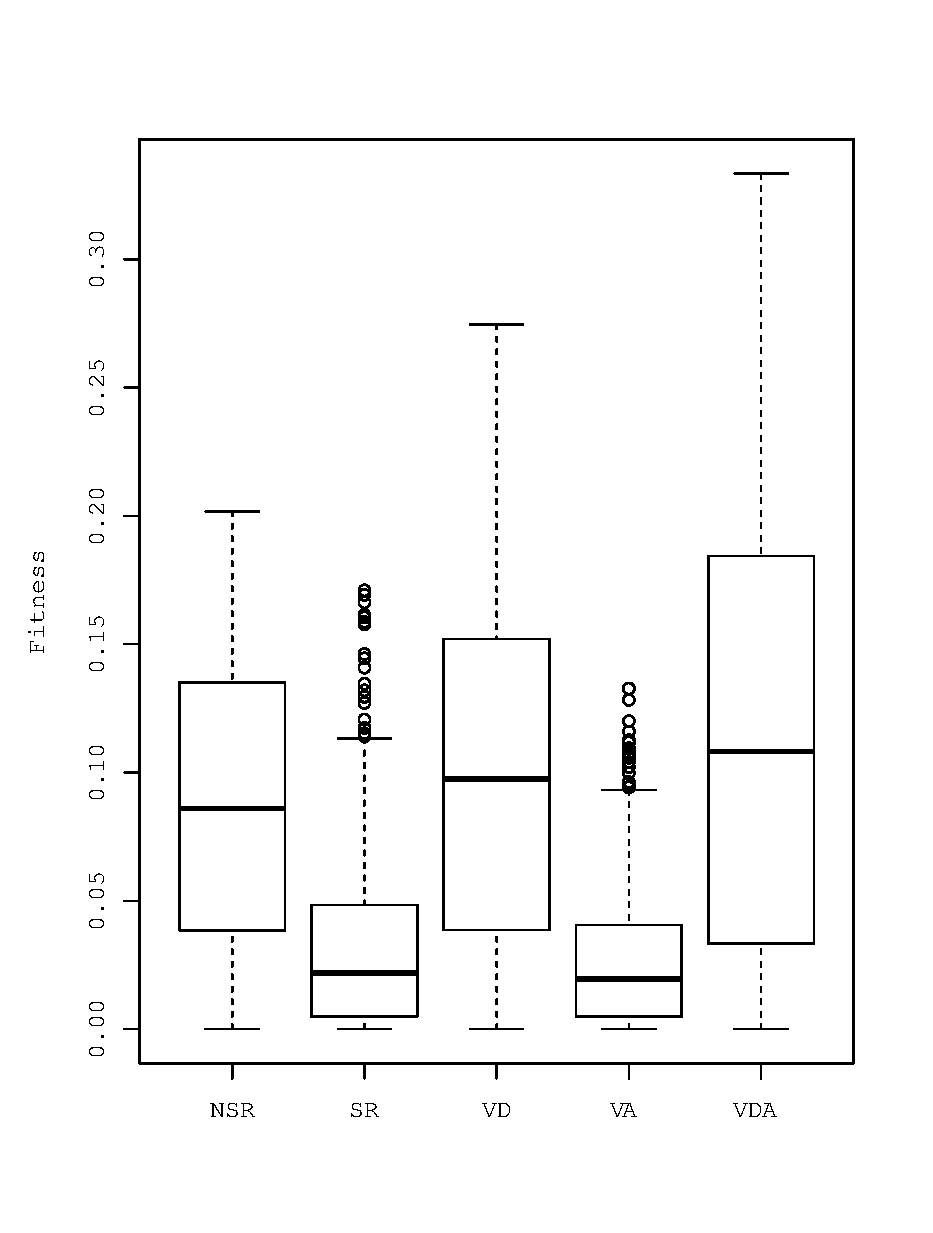
\includegraphics[width=\textwidth]{figures/reeval-nsr}
        \subcaption{NSR}
        \label{fig:reeval-nsr}
    \end{minipage}%
    \quad
    \begin{minipage}{.4\textwidth}
        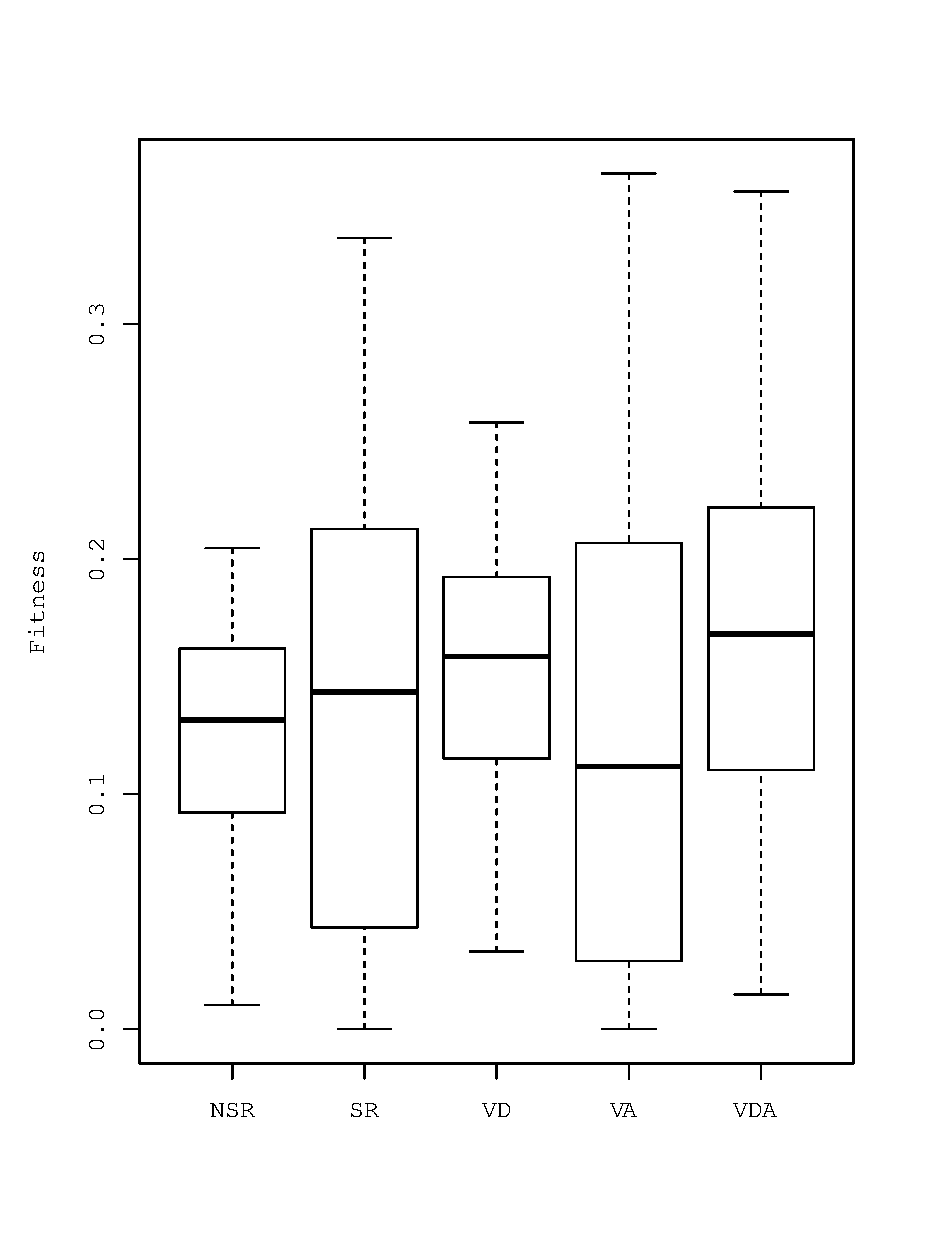
\includegraphics[width=\textwidth]{figures/reeval-sr}
        \subcaption{SR}
        \label{fig:reeval-sr}
    \end{minipage}

    \caption{Reavaliações}
\end{figure}

\begin{figure}[h]
    \centering
    \begin{minipage}{.5\textwidth}
        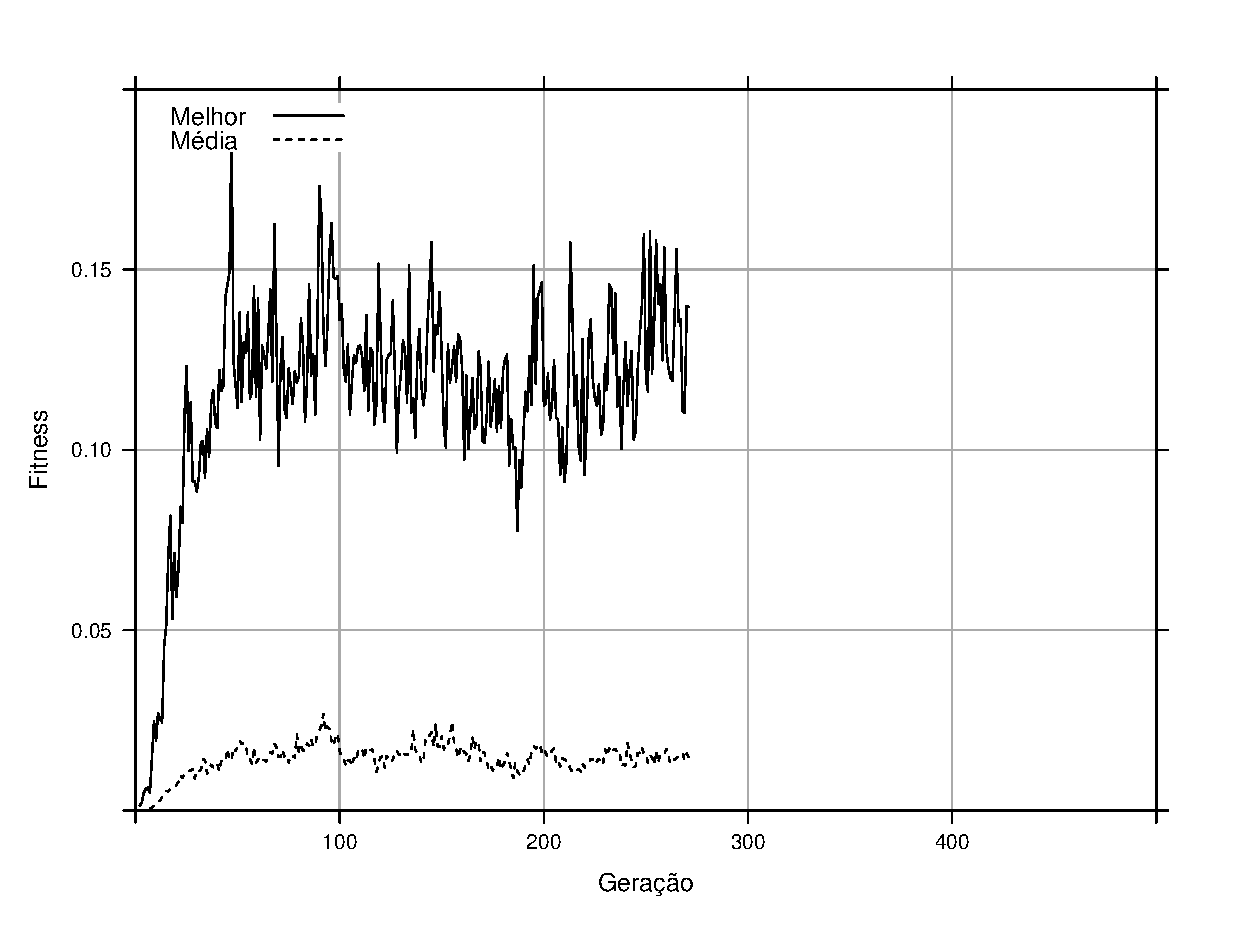
\includegraphics[width=\textwidth]{figures/fitness-GA}
        \subcaption{GA}
    \end{minipage}%
    \begin{minipage}{.5\textwidth}
        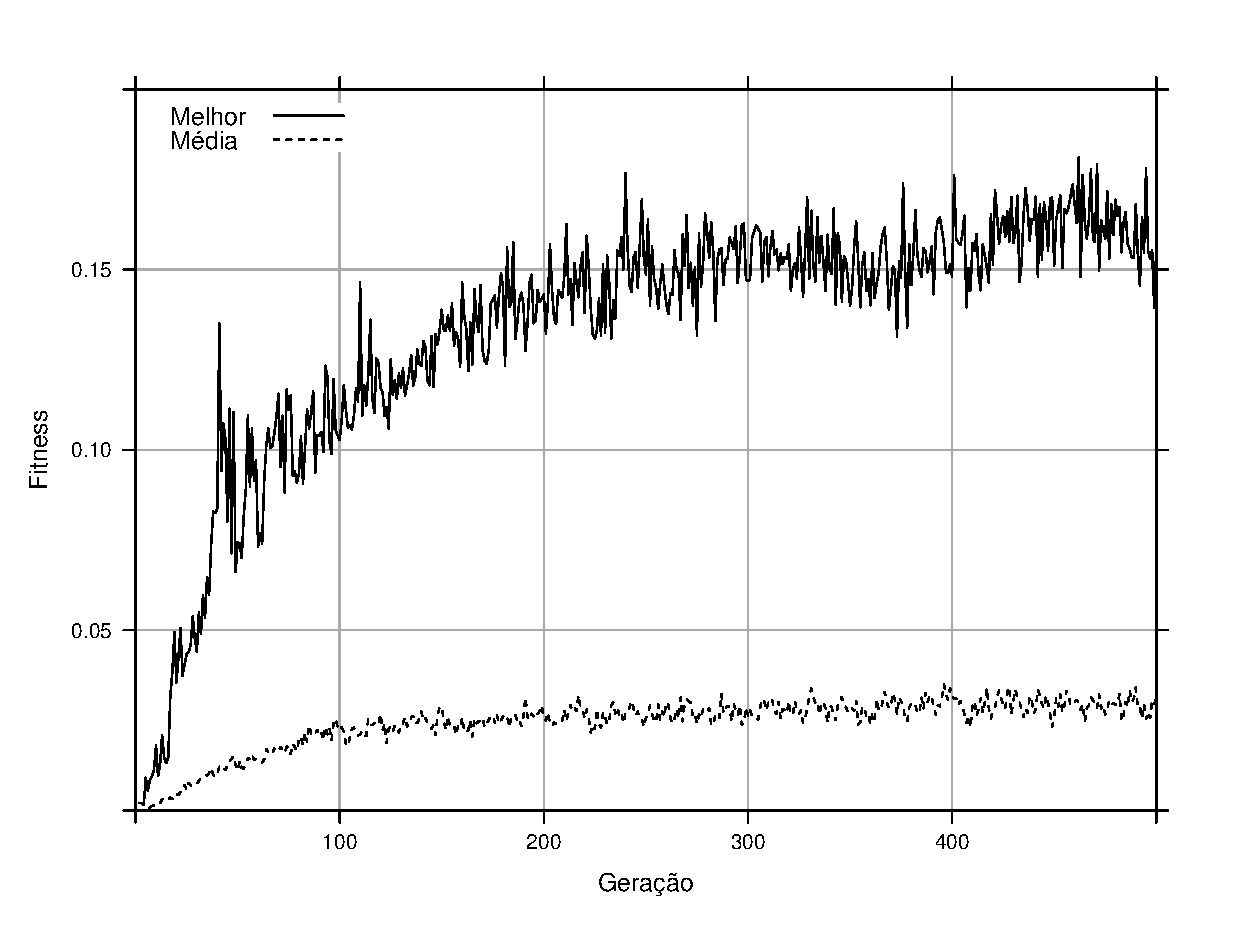
\includegraphics[width=\textwidth]{figures/fitness-PGA}
        \subcaption{CGPGA}
    \end{minipage}

    \begin{minipage}{.5\textwidth}
        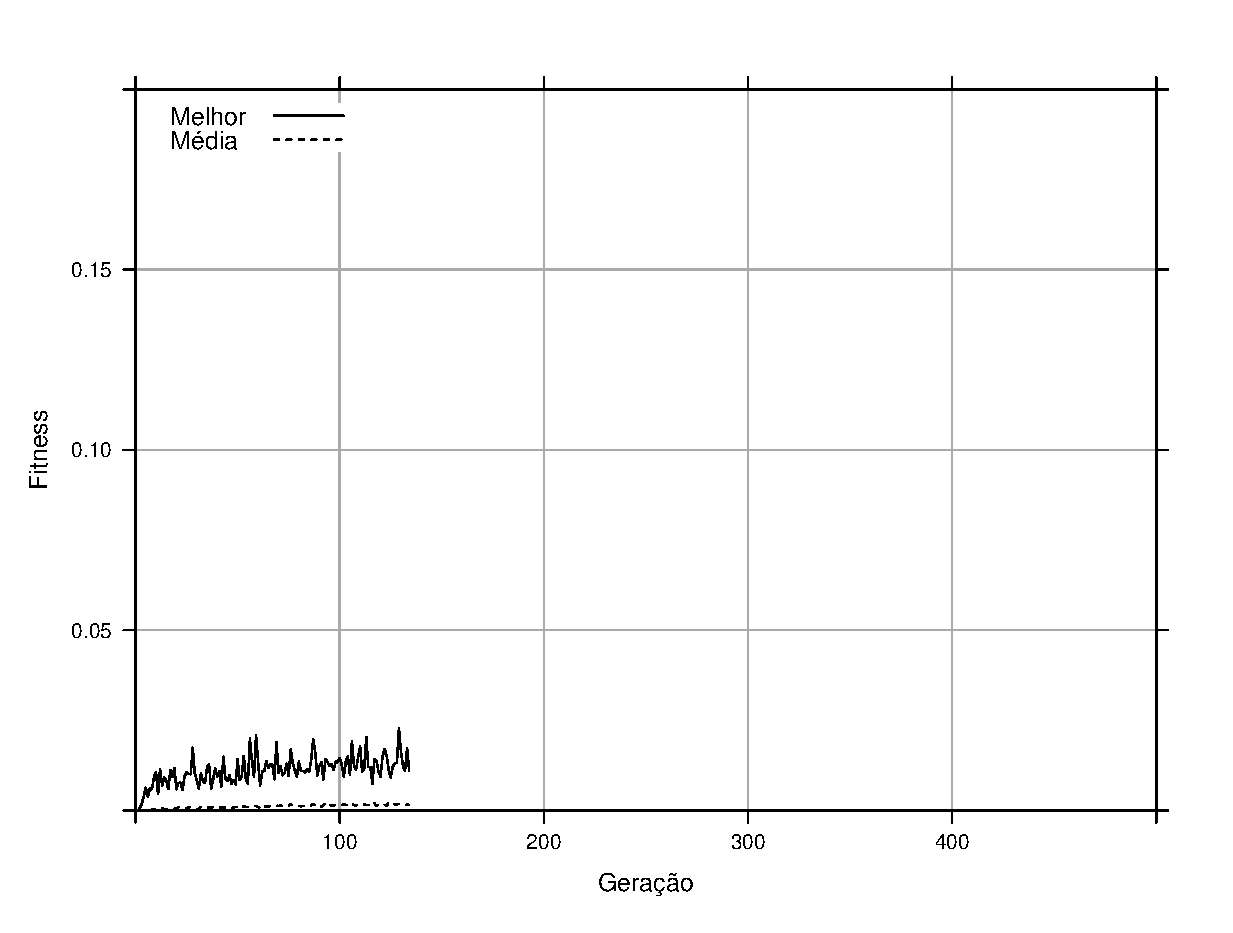
\includegraphics[width=\textwidth]{figures/fitness-PSO}
        \subcaption{PSO}
    \end{minipage}%
    \begin{minipage}{.5\textwidth}
        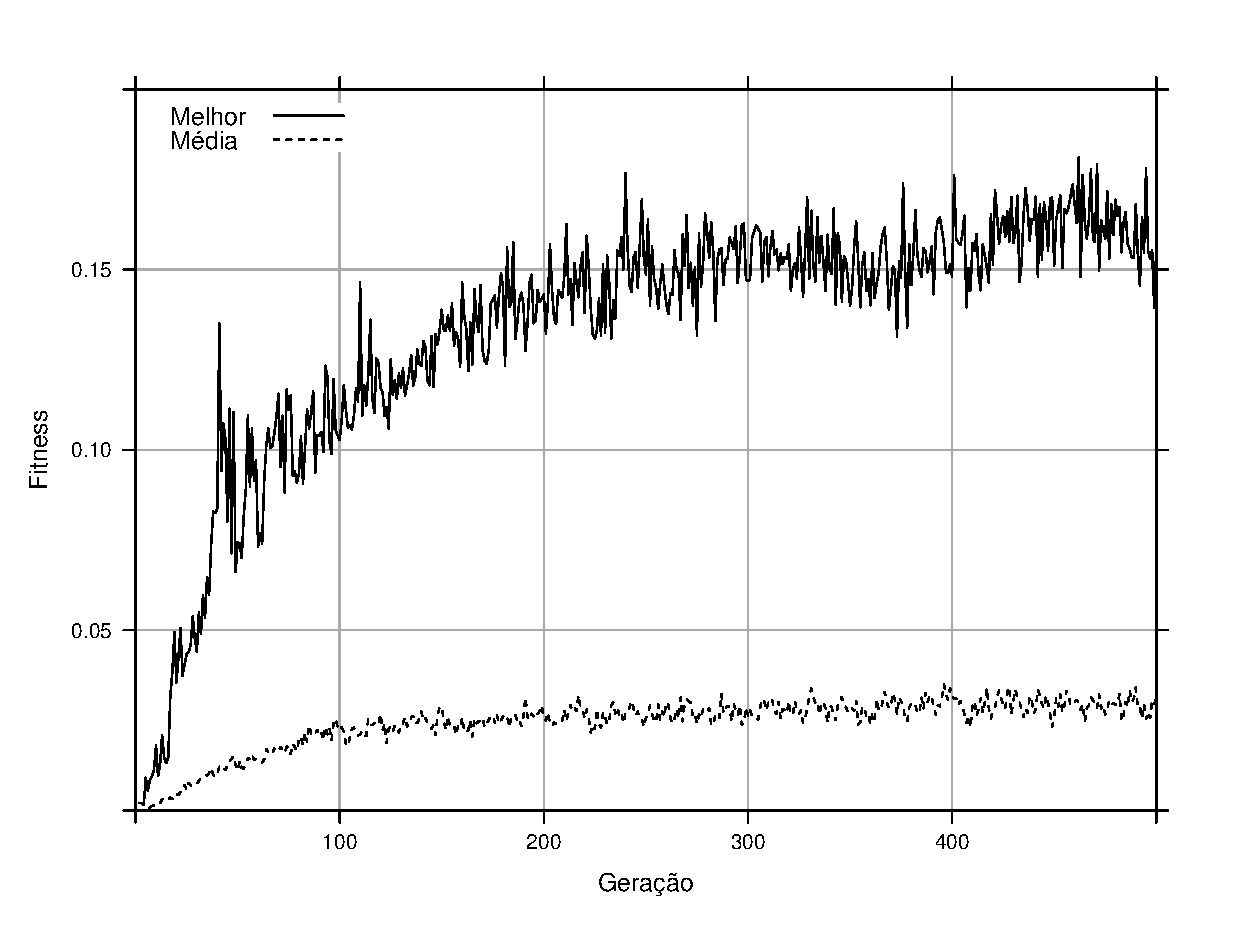
\includegraphics[width=\textwidth]{figures/fitness-PGA}
        \subcaption{DPSO}
    \end{minipage}

    \caption{Fitness}
\end{figure}
\chapter{Conclusão}
\label{conclusao}

\bibliographystyle{brazil}
\bibliography{referencias}
% utilize macros (3 primeiras letras do mes em ingles, minusculas) no seu
% .bib para atribuir o nome do mes em portugues nas referencia,
% se o style for brazil, outros estilos tambem aceitam estas macros
% Ex:
%
% @InProceedings{teste,
%   author =       {Luciano}
%   year =         {2000}
%   month =        {}#sep;
% }

\addcontentsline{toc}{chapter}{BIBLIOGRAFIA}

\end{document}